\documentclass{article}

\usepackage{graphicx}
\usepackage{cite}
\usepackage{amssymb}
\usepackage{amsmath}
\usepackage{listings}
\usepackage{color}
\usepackage[section]{placeins}

\definecolor{dkgreen}{rgb}{0,0.6,0}
\definecolor{gray}{rgb}{0.5,0.5,0.5}
\definecolor{mauve}{rgb}{0.58,0,0.82}

\lstset{frame=tb,
  language=python,
  aboveskip=3mm,
  belowskip=3mm,
  showstringspaces=false,
  columns=flexible,
  basicstyle={\small\ttfamily},
  numbers=none,
  numberstyle=\tiny\color{gray},
  keywordstyle=\color{blue},
  commentstyle=\color{dkgreen},
  stringstyle=\color{mauve},
  breaklines=true,
  breakatwhitespace=true,
  tabsize=3
}

\begin{document}
\section{Winding Number Algorithm}
The winding number algorithm was the algorithm that we first built to test insideness.
Let $C$ represent a polygon with $n$ vertices.
Let $V_i$ be a vertex of $C$ where $1$ $\leq$ $i$ $\leq$ $n$.
We define the winding number as a function $W(P,C)$ where $P$ is a point and $C$ is a polygon.
$$
W(P,C) = \frac{1}{2\pi}\sum_{i=1}^{n-1}\arccos{\frac{(V_i-P)\cdot (V_{i+1}-P)}{|V_i-P||V_{i+1}-P|}}.
$$
A point $P$ is inside the polygon $C$, if $W(P,C) \not= 0$.
The winding number has a simple implementation from a coding perspective and is very accurate.
Issues arise with speed, the winding number requires the use of $arccos$ which is computationaly expensive.

\section{Ray Casting Algorithm}

The ray casting algorithm at its core works by taking a given point $Q$ and extending that point in the positive $x$ direction.
Let us refer  to that ray $\overrightarrow{\rm Q}$.
If $Q = (a,b)$, then $\overrightarrow{\rm Q} = \{ a + x | \; x \geq 0, x \in \mathbb{R} \}$ where $x \in \mathbb{R}$.
Let $C$ be a polygon with $n$ vertices, each line segement formed by connecting vertices we consider to be edges.
If $Q$ lies outside the polygon, the $\overrightarrow{\rm Q}$ will either not intersect the polygon at all, or there will be at least two intersections.
To keep track of how many times a point passes through a polygon we increment the intersection index.
We define the intersection index $I$ as a iterator of how many times an extended ray $\overrightarrow{\rm Q}$ intersects the polygon $C$.
\FloatBarrier
\begin{figure}[!h]
	\center{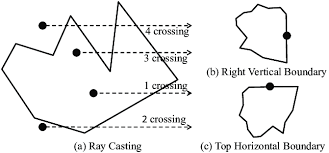
\includegraphics[width=0.5\textwidth]{Figures/bbimplmentation.png}}
	  \vspace{0in}
	  \caption{\label{fig:raycasting} Visualization of the crossings}
\end{figure}
\FloatBarrier
If $I$ is even the point is outside the polygon.
If $I$ is odd the point is inside the polygon.
By example, $I$ is displayed in figure \ref{fig:raycasting}.


\subsection{Crossing Number Implementation of Ray-Casting}
The crossing number algorithm and all other ray-casting inspired algoirthms are considered applicable to all polygons\cite{arb_polys}.
The winding number depends on floating point numbers to preform the calculations\cite{arb_polys}.
This could be considered a weakness as the variable typings create more memory than they should.
I will discuss this weakness of the winding number in the optimization section.
For now, let us define the crossing number algorithm.

The first thing we are going to define is the mathematical significance of the crossing number.
To begin, let us discuss the similarities between the Ray Casting Algorithm and the Crossing Number algorithm.
They both use this idea of extending a point into a ray.
Let $P=(a,b)$ be a point in euclidean space such that $a,b\in \mathbb{R}$.
Let us now define a function $CN$ that takes an edge of the curve $E_i$ and $P$ as inputs.
Let $E_i = (V_i, V_{i+1})$ where $V_i$ are vertices from the polygon $C$.
We reference the points that define the edge like $E_i.V_2 \; \textrm{and} \; E_i.V_2$.
Firstly, we check to see if $P.y$ or $P.x$ are within greater than the mins and less than the maxs.
If that statement is true, we test to see if it crosses the particular edge,
$$
    \textrm{Let d = $\frac{P.y-E_i.V_1.y}{E_{i}.V_2.y - E_i.V_1.y}$.}
$$
$$
    CN(E_i,P) =\left\{
                \begin{array}{ll}
                    0 & \quad  P.x \geq E_i.V_1.x + d*(E_i.V_2.x - E_i.V_1.x)\\
                    1 & \quad P.x < E_i.V_1.x + d*(E_i.V_2.x - E_i.V_1.x)
                \end{array}
            \right.
$$.
For each vertex of the arbitrary polygon $C$ the crossing number is computed for each vertex.
The insideness of the point is determined by the intersection index.
The intersection index $I$ is also slightly different to the deffinition that ray-casting uses.
$$
    I = \sum_{i=1}^{n-1} CN(P,E_i) + CN(P, E_{i+1})
$$
$P$ is inside the polygon if $I$ is an odd number and is outside the polygon if $I$ is even.
The idea of ray-casting stays the same amongst the crossing number.
What I mean is, crossing number and ray-casting ``cancel'' out edges based on how $\overrightarrow{\rm Q}$ collides with $C$.
We choose to calculate the collisons $\overrightarrow{\rm Q}$ makes with the polygon by incorporating a sense of direction of the ray.
There are other implementations that sum $I$ differently depending on the circumstances of the polygon.




\subsection{Optimization of the Crossing Number}
We discussed earlier the bounding box implementation.
To summerize, the bounding box implementation we discussed counts the amount of entries vs the amount exits and determines if the point is inside the space or not.
If the number is an even number of crossings, the point is outside the polygon.
If there is an odd number of crossings, the point is inside the figure.
When we say "crossings", we are talking about the amount of times that a ray extends in the positive x-axis from the point give intersects the polygon.
The bounding box amd crossing numberm in general, the same.
So what are the differences?
The main differences stem from their implementations.
Firstly lets look both algorithms in the python code.

\begin{lstlisting}
@njit(parallel=True)
def bounding_box_algorithm(domain, p, prior_intersections, min_max):
    intersections = prior_intersections
    left_int = False
    right_int = False
    last_intersection = 0
    x_max = min_max[0]
    y_max = min_max[1]
    x_min = min_max[2]
    y_min = min_max[3]
    y_tolerence = .00000001

    if p[0] < x_min or p[1] < y_min:
        return None
            
    if p[0] > x_max or p[1] > y_max:
        return None

    for pos in range(0,len(domain)):
        if pos < len(domain)-1:
            point_1 = domain[pos]
            point_2 = domain[pos+1]

            w = point_1
            v = point_2
        
            w_v = (w[0]-v[0], w[1]- v[1])
            p_v = (v[0]-p[0], v[1]-p[1])
            p_w = (w[0]-p[0], w[1]-p[1])
            
            dot_prod = float(w_v[0] * p_v[0] + w_v[1]*p_v[1])

            # if not_rad > 170 and dot_prod < 1 and dot_prod > -1:
            #     continue

            if v[1] <= p[1] and p[1] < w[1] and dot_prod > 0:
                intersections += 1

            elif w[1] <= p[1] and p[1] < v[1] and dot_prod <= 0:
                intersections -=1

    return intersections

\end{lstlisting}

\begin{lstlisting}
@njit(parallel=True)
def crossing_number(domain, p, cn):

    for i in range(0,len(domain)-1):
        edge = (domain[i], domain[i+1])
        
        if (edge[0][1] <= p[1] and edge[1][1] > p[1]) or (edge[0][1] > p[1] and edge[1][1] <= p[1]):
            vt = float(p[1] - edge[0][1]) / float(edge[1][1] - edge[0][1])
            if p[0] < edge[0][0] + vt * (edge[1][0] - edge[0][0]): 
                cn += 1

    return cn

\end{lstlisting}

The difference in length is staggering, especially because they are in a sense the same thing.
What I want to focus on here is how in the bounding box implementation we use rays rather directly.
Whereas, with the crossing number, we don't do as many operations.
We just compare and divide floats given to the function.
We also do not subtract intersections.
The subtracting of intersections could have been one of the causes for the innaccuracies of the algorithm.
I believe that the main cause was the handeling of the numbers.
In the bounding box algorithm we also define a lot of variables, these deffinitions of could have impacted the accuracy of the numbers.


Before we can discuss the innaccuracies of the numbers we need to discuss what the Njit line above the functions mean.
That line is called a decorator.
A decorator tells the compiler to reinterpret the function based on what the decorator has in store.
In our case, the Njit line dictates to the compiler that the functions are set to be compiled in a more C fashion.
In other words, typings are now enforced.
Typing is used to tell the compiler how many bits each variable will neeed.
In C types are supposed to be explicitly defined before using the variables the user defines.
Whereas, in python, that concept does not exist.
Python defines the typing of variables based on the context of the code.
It's a very impressive technique, many languages have adopted this methodology for compiling their variables.
Without typing, code can be writen in a more abstract way.
The extra layer of abstraction makes programming simpler and faster to do.
As nice as it sounds, there are drawbacks.
The biggest one being speed.
If the compiler handels all of the typings of variables, they have to almost guess.
The fact they have to pretty much guess, means there are a lot of checks as to what variable will work.
To make sure they are absolutly sure, the compiler does a lot of tests at runtime before running the code.
If the cannot figure out what the variable is, the user will get an error while running the code.
This is suppose to act as a check to ensure we don't break the code.
Typing variables is important to programers as it determines how many bits the variable will need to be represented.
Having more control over variables puts more responsibility on the programmer to know what they are doing.
Typing also allows for the code to run faster.
What I mean is there are less safety checks at runtime, less checking allows for code to be executed much faster.
So, Njit allows use to take advantage the speed of C while retaining the abstractness python inherently gives.

How does Njit impact the numbers within our algorithms?
Njit doesn't know if a number is an integer or a double.
This is important because doubles use more bits than integers.
If you notice, the bounding box algorithm does many more operations with given values.
This means there are more chances where the compiler misinterprets the numbers for being different things.
If the compiler interprets the output of multiplication of an integer and a double as a integer, we lose a lot of data the double once held.
Therefore, the bounding box algorithm has more of a change to lose data.





\bibliography{Algorithm_writeup}{}
\bibliographystyle{plain}
\end{document}